\renewcommand{\thesubsection}{\textcolor{red}{\Roman{section}.\arabic{subsection}}}
\renewcommand{\thesubsubsection}{\textcolor{red}{\Roman{section}.\arabic{subsection}.\alph{subsubsection}}}

\setcounter{section}{0}
\sndEnTeteCoursDeux

\begin{mdframed}[style=titr, leftmargin=60pt, rightmargin=60pt, innertopmargin=7pt, innerbottommargin=7pt, innerrightmargin=8pt, innerleftmargin=8pt]

\begin{center}
\large{\textbf{Chapitre 2 : Les solutions aqueuses}}
\end{center}
\end{mdframed}
Dans ce chapitre, nous nous intéressons à un type de mélanges homogènes en particulier : les solutions aqueuses. 

\begin{tcolorbox}[colback=blue!5!white,colframe=blue!75!black,title=Mots clés du chapitre :]
Solution, solvant, soluté, solubilité, dissolution, dilution, échelle de teinte, courbe d'étalonnage. 
\end{tcolorbox}


\section{Composition d'une solution}
\begin{Large}
    \ding{43}
\end{Large}\textit{Voir activité 1 : Concentration en masse}
\begin{tcolorbox}[colback=green!5!white,colframe=green!75!black,title=\textbf{Solution, solvant, soluté}]
\begin{center}
    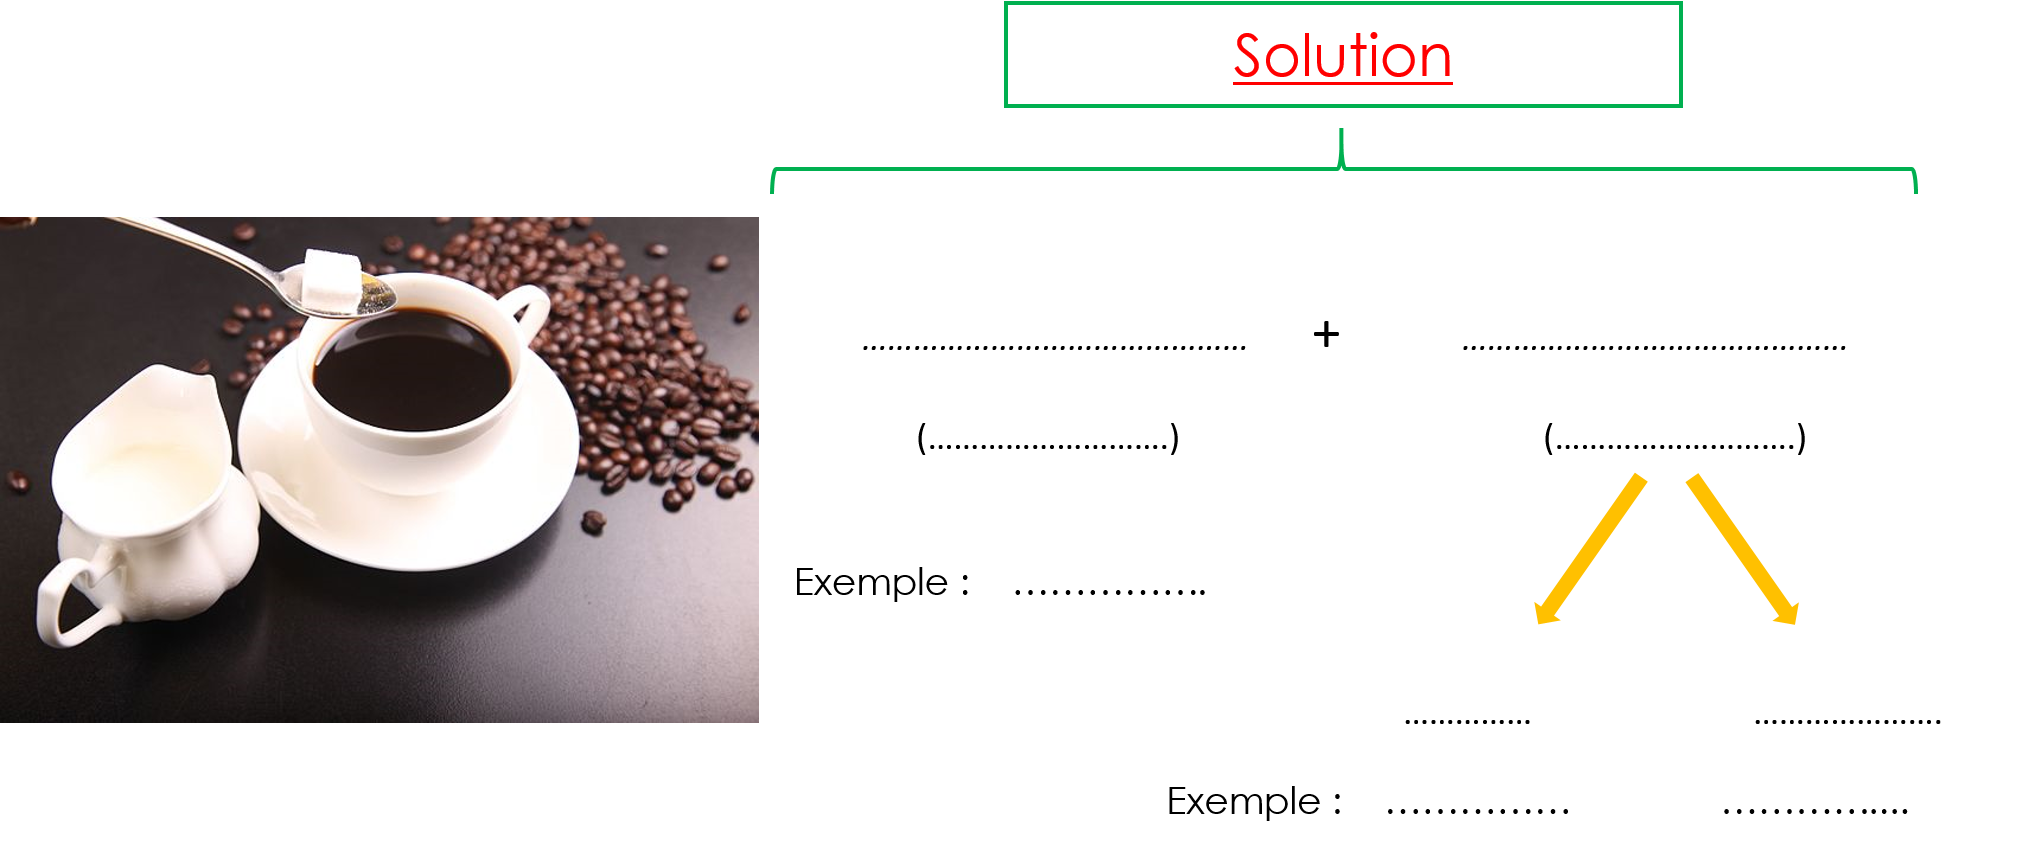
\includegraphics[width=\textwidth]{Images/Solution_def.png}
\end{center}
\end{tcolorbox}
Sur l'image de la tasse de café ci-dessus, qui jouent le rôle du solvant et des solutés ? Comment s'appelle la solution ?\\
\textit{Réponse :} \gap{........................................................................................................................}\\

\begin{Large}
    \ding{45}
\end{Large}\textbf{Exercice DOC : l'alcool dénaturé.}
\section{Concentration en masse et solubilité}
\subsection{Concentration en masse}
\begin{tcolorbox}[colback=green!5!white,colframe=green!75!black,title=\textbf{Définition}, upperbox=invisible]
La concentration en masse d’un soluté dans une 
solution est la masse de soluté dissous $m_{\text{soluté}}$ par rapport au volume de solution $V_{\text{solution}}$ :
\begin{equation*}
    C_m = \frac{m_{\text{soluté}}}{V_{\text{solution}}}
\end{equation*}
Elle est notée $C_m$ et elle s’exprime en gramme par litre (\textbf{g.L$^{-1}$}).
\end{tcolorbox}

\importantbox{
\begin{Large}
    \ding{43}
\end{Large}\textit{Voir activité 1 : Concentration en masse}
\begin{empheq}[box=\fbox]{equation*}
    C_m = \frac{m_{\text{soluté}}}{V_{\text{solution}}} \neq \rho = \frac{m_{\text{solution}}}{V_{\text{solution}}}
\end{empheq}
}
\begin{Large}
    \ding{45}
\end{Large}\textit{Exercices 14, 15, 25}\\

\textcolor{blue}{\textbf{Remarque :}} Peut-on ajouter une quantité infinie de soluté dans un solvant ? Non bien sûr, il existe une quantité maximale de soluté qu'on peut dissoudre dans un solvant : c'est la solubilité.
\subsection{Solubilité}
Comprendre la solubilité en vidéo : \url{https://www.youtube.com/watch?v=8bkfkRu_mbg}\\
\begin{Large}
    \faFlask
\end{Large} \textcolor{blue}{\textbf{Expérience :}} Dissolution de sel dans l'eau et dans l'huile.
\begin{tcolorbox}[colback=green!5!white,colframe=green!75!black,title=\textbf{Définition}, upperbox=invisible]
La solubilité, notée $s$, d'une espèce chimique est la masse maximale de cette espèce que l'on peut dissoudre dans $1$~L de solvant. Elle s'exprime en $\mathbf{g.L^{-1}}$.\\
Il s'agit d'une \textbf{concentration massique} !\\

La solubilité d'un soluté particulier dépend : 
\begin{center}
   1. de la température,\\
   2. du solvant utilisé.
\end{center}
\end{tcolorbox}

\section{Préparer des solutions aqueuses}

\subsection{Préparer par dissolution}
Le principe est de dissoudre une certaine masse de soluté (en général, il s'agit d'un solide) dans un volume précis d'eau afin d'obtenir une solution aqueuse de concentration en masse de soluté bien précise.

\begin{tcolorbox}[colback=red!5!white,colframe=red!75!black,title=\textbf{Protocole de préparation de la dissolution (résumé) : }, upperbox=invisible]
    \vspace{10cm}
\end{tcolorbox}


\begin{mdframed}[style=autreexo]
\textbf{\bsc{Exercice de cours} - Dissolution}\\
On souhaite préparer par dissolution 100 mL d’une solution aqueuse de concentration en masse de sulfate de cuivre égale à 15 g.L$^{-1}$. Calculer la masse de soluté à peser.\end{mdframed}
\gap{.......................................................................................................................................}
\newline
\gap{.......................................................................................................................................}\\
\begin{Large}
    \ding{45}
\end{Large}\textit{Exercice 18}

\subsection{Préparer par dilution}
Le principe est de prélever un certain volume d'une solution concentrée initiale appelée \textcolor{red}{solution mère} puis d'y ajouter de l'eau pour obtenir une solution moins concentrée appelée \textcolor{red}{solution fille} :
\begin{center}
    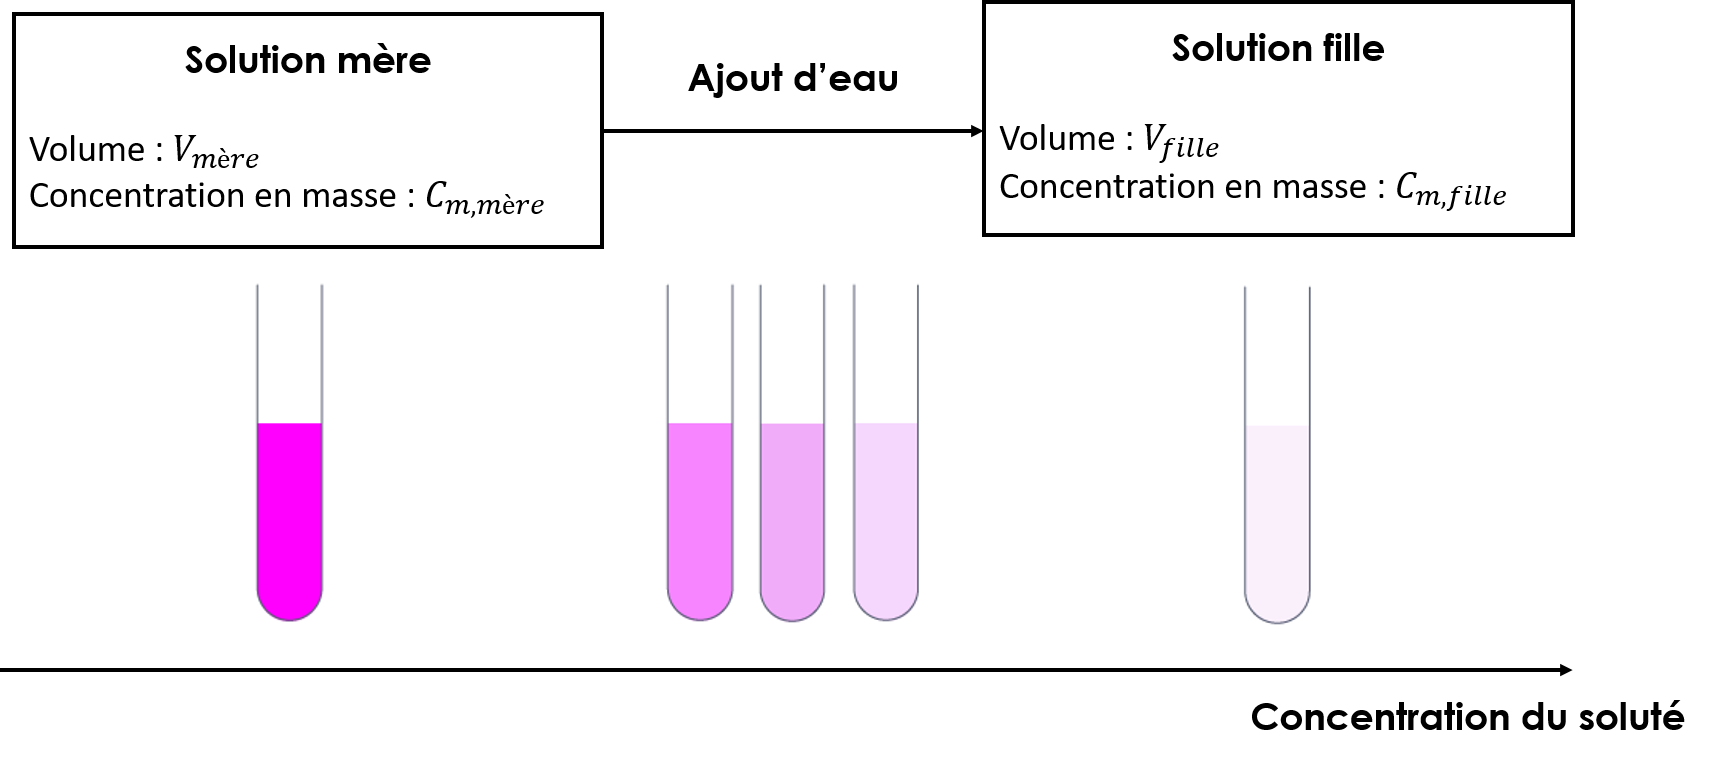
\includegraphics[scale=0.59]{Images/Dilution.png}
\end{center}
\begin{tcolorbox}[colback=red!5!white,colframe=red!75!black,title=\textbf{Propriété de la dilution : }, upperbox=invisible]
Au cours d'une dilution, la masse de soluté prélevée se conserve :
\begin{empheq}[box=\fbox]{align*}
    m_{\text{prélevée, mère}} &= m_{\text{soluté, fille}}\\
    C_{m,\text{mère}}V_{\text{prélevé}} &= C_{m,fille}V_{\text{fille}}
\end{empheq}
On peut dès lors définir le \textcolor{red}{facteur de dilution}, noté $F$ de la manière suivante :
\begin{equation*}
    F=\frac{C_{m,\text{mère}}}{C_{m,fille}} = \frac{V_{\text{fille}}}{V_{\text{prélevé}}}
\end{equation*}
\end{tcolorbox}
\begin{center}
    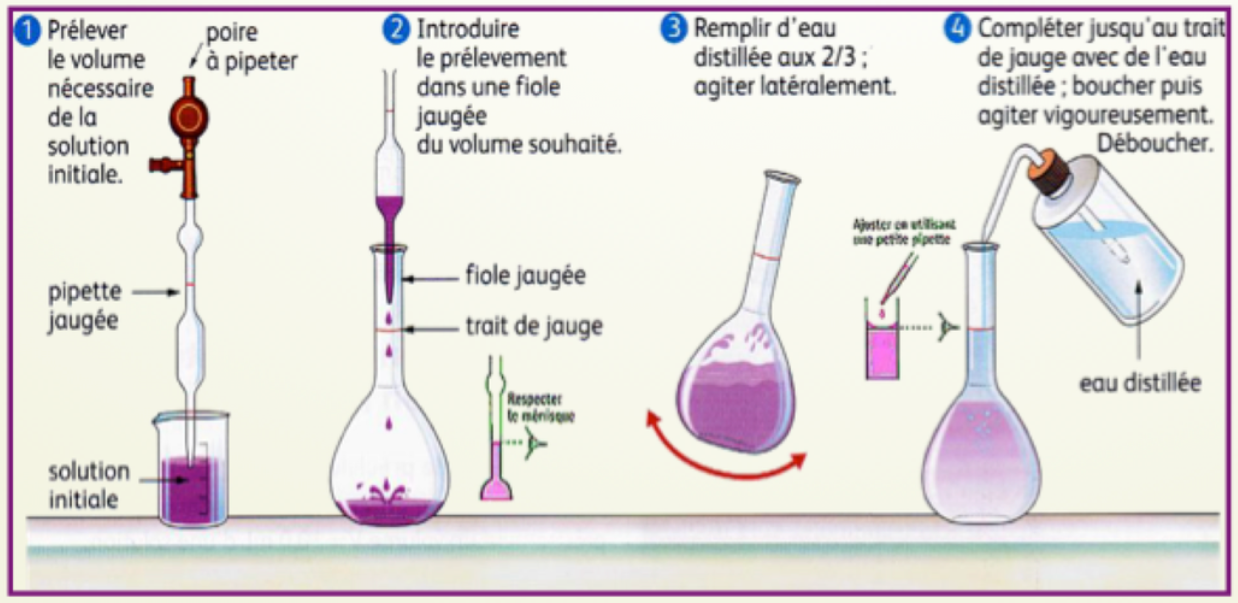
\includegraphics[scale=0.6]{Images/Protocole_dilution.png}
\end{center}

Avant de préparer une solution aqueuse par  dilution, il faut calculer le volume $V_{\text{mère}}$ de solution mère à 
prélever.\\

\begin{mdframed}[style=autreexo]
\textbf{\bsc{Exercice de cours} - Dilution}\\
On souhaite préparer par dilution 100 mL d’une solution aqueuse de concentration en masse de sulfate de cuivre égale à 15 g.L$^{-1}$ à partir d’une solution aqueuse de concentration en masse de sulfate de cuivre égale à 60 g.L$^{-1}$. Calculer le volume de solution mère à prélever. Calculer le facteur de dilution $F$.
\end{mdframed}

\gap{.......................................................................................................................................}
\newline
\gap{.......................................................................................................................................}
\newline
\gap{.......................................................................................................................................}
\newline
\gap{.......................................................................................................................................}\\

\begin{Large}
    \ding{45}
\end{Large}\textit{Exercices 16, 21}
\section{Détermination de la concentration en masse d'une solution}

\subsection{Echelle de teinte}
\begin{Large}
    \ding{43}
\end{Large}\textit{Voir TP : Préparer un médicament par dilution}\\
Partons de l'exemple suivant : on peut savoir si un verre de sirop dilué par de l'eau est plus ou moins concentré en sirop, simplement en regardant la couleur du mélange par rapport à la couleur du sirop sans eau. En faisant cela, on réalise sans le savoir une \textcolor{red}{échelle de teinte}. La solution diluée est appelée \textcolor{red}{solution étalon}.\\
En chimie, l'utilisation d'une échelle de teinte permet \textbf{d'encadrer la valeur d'une concentration en masse d'un soluté coloré}. Regardons la figure suivante :

\begin{center}
    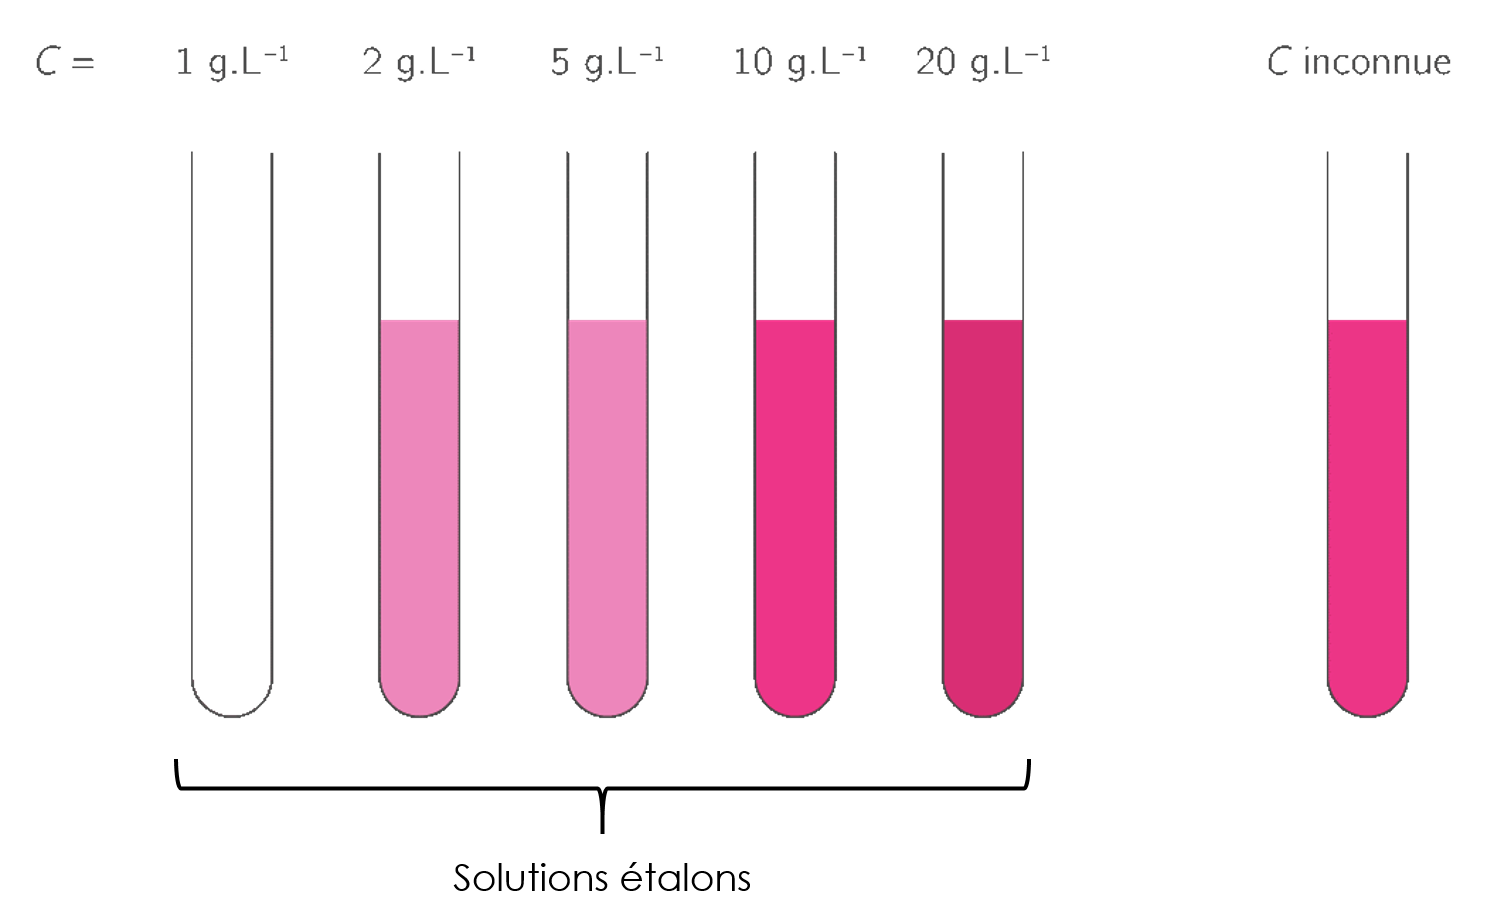
\includegraphics[scale=0.45]{Images/Echelle_teinte.png}
\end{center}

\begin{mdframed}[style=autreexo]
\textbf{\bsc{Exercice de cours} - Echelle de teinte}\\
Encadrer la concentration $C_{inconnue}$ en visualisant l'écchelle de teinte réalisée ci-dessus.
\end{mdframed}


\subsection{Par une courbe d'étalonnage}
\begin{Large}
    \ding{43}
\end{Large}\textit{Voir TP : Les sodas sont-ils très sucrés ?}\\
Une deuxième méthode plus précise consiste à réaliser une \textcolor{red}{courbe d'étalonnage} d'une grandeur physique ou chimique (par exemple : la masse volumique $\rho$, la conductivité $\sigma$, l'absorbance $A$ d'une solution, etc) à partir des solutions étalons.

\begin{center}
    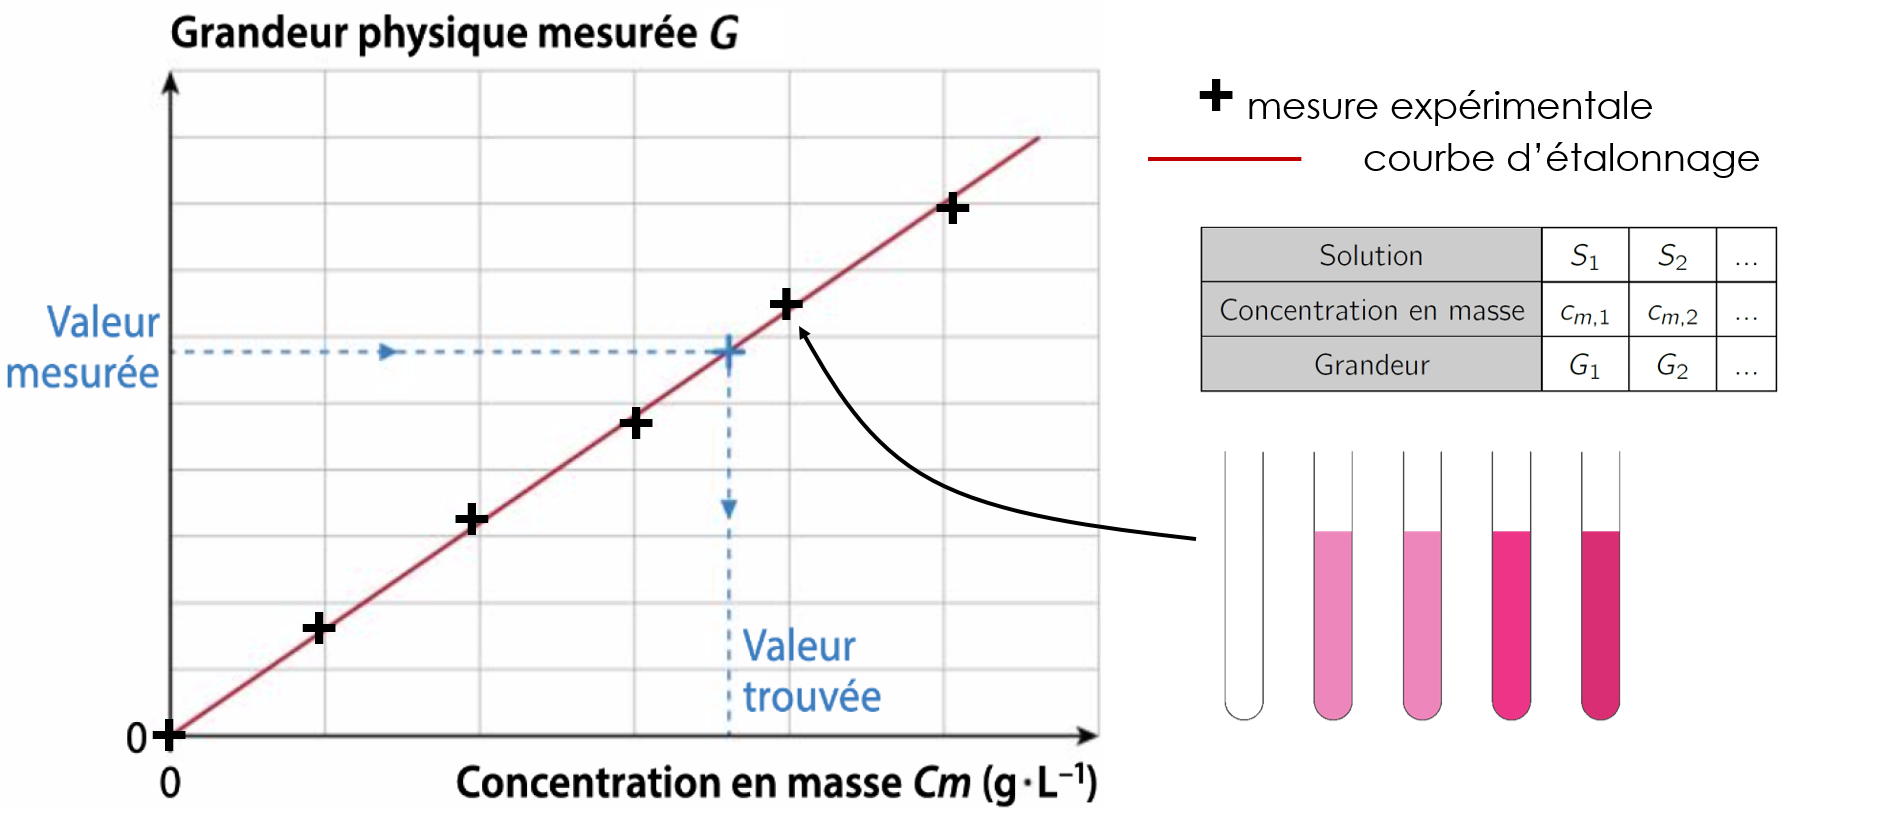
\includegraphics[scale=0.6]{Images/Courbe_etalonnage.png}
\end{center}

\begin{tcolorbox}[colback=red!5!white,colframe=red!75!black,title=\textbf{Protocole expérimental pour réaliser une courbe d'étalonnage: }, upperbox=invisible]
\begin{enumerate}
    \item Préparer une série de solutions étalons, c’est-à-dire des solutions obtenues à partir du même soluté que la solution de concentration inconnue et dont les concentrations en masse sont connues,
    \item Mesurer la valeur de la grandeur G pour chacune des solutions étalons,
    \item À partir des mesures précédentes, tracer la courbe représentant la grandeur $G$ en fonction de la concentration en masse $C_m$, appelée courbe d’étalonnage,
    \item Lorsque la grandeur $G$ est proportionnelle à concentration en masse $C_m$, la courbe d’étalonnage est une droite qui passe par l’origine,
    \item Mesurer la valeur de la grandeur $G$ pour la solution de concentration inconnue,
    \item Déterminer la concentration inconnue par lecture graphique sur la courbe d’étalonnage.
\end{enumerate}
\end{tcolorbox}